\documentclass[11pt,a4paper,notitlepage]{article}
\usepackage[utf8]{inputenc}
\usepackage[english]{babel}
\usepackage{amsmath}
%\usepackage{indentfirst}
\usepackage{amsfonts}
\usepackage{amssymb}
\usepackage{makeidx}
\usepackage{titlesec}
\usepackage{graphicx}
\usepackage{caption}
\usepackage{subcaption}
\usepackage{float}
\usepackage[left=2cm,right=2cm,top=2cm,bottom=2cm]{geometry}
\usepackage{fancyvrb}
\DefineVerbatimEnvironment{code}{Verbatim}{fontsize=\small}
\DefineVerbatimEnvironment{example}{Verbatim}{fontsize=\small}

\def\TeX{{\rm T\kern-.1667em\lower.5ex\hbox{E}\kern-.125emX}}

\title{FeyPy: A Python package for visualizing and calculating nonlinear optical properties}

\author{Team Cobra, Washington State University}

\begin{document}

\maketitle

\section{Features}

FeyPy is an object-oriented Python package. The programming objective for this package was to construct a framework for visualizing complicated nonlinear optical processes using a Feynman diagram approach and then to use those visualizations to calculate useful properties of such systems, such as the overall nonlinear response of a series of molecules interactive via optical cascading. Other useful things, such as $\LaTeX$ strings and the ability to fit data to an expected nonlinear process are also implemented.

\section{Package Directory}

\begin{figure}[htb]
\centering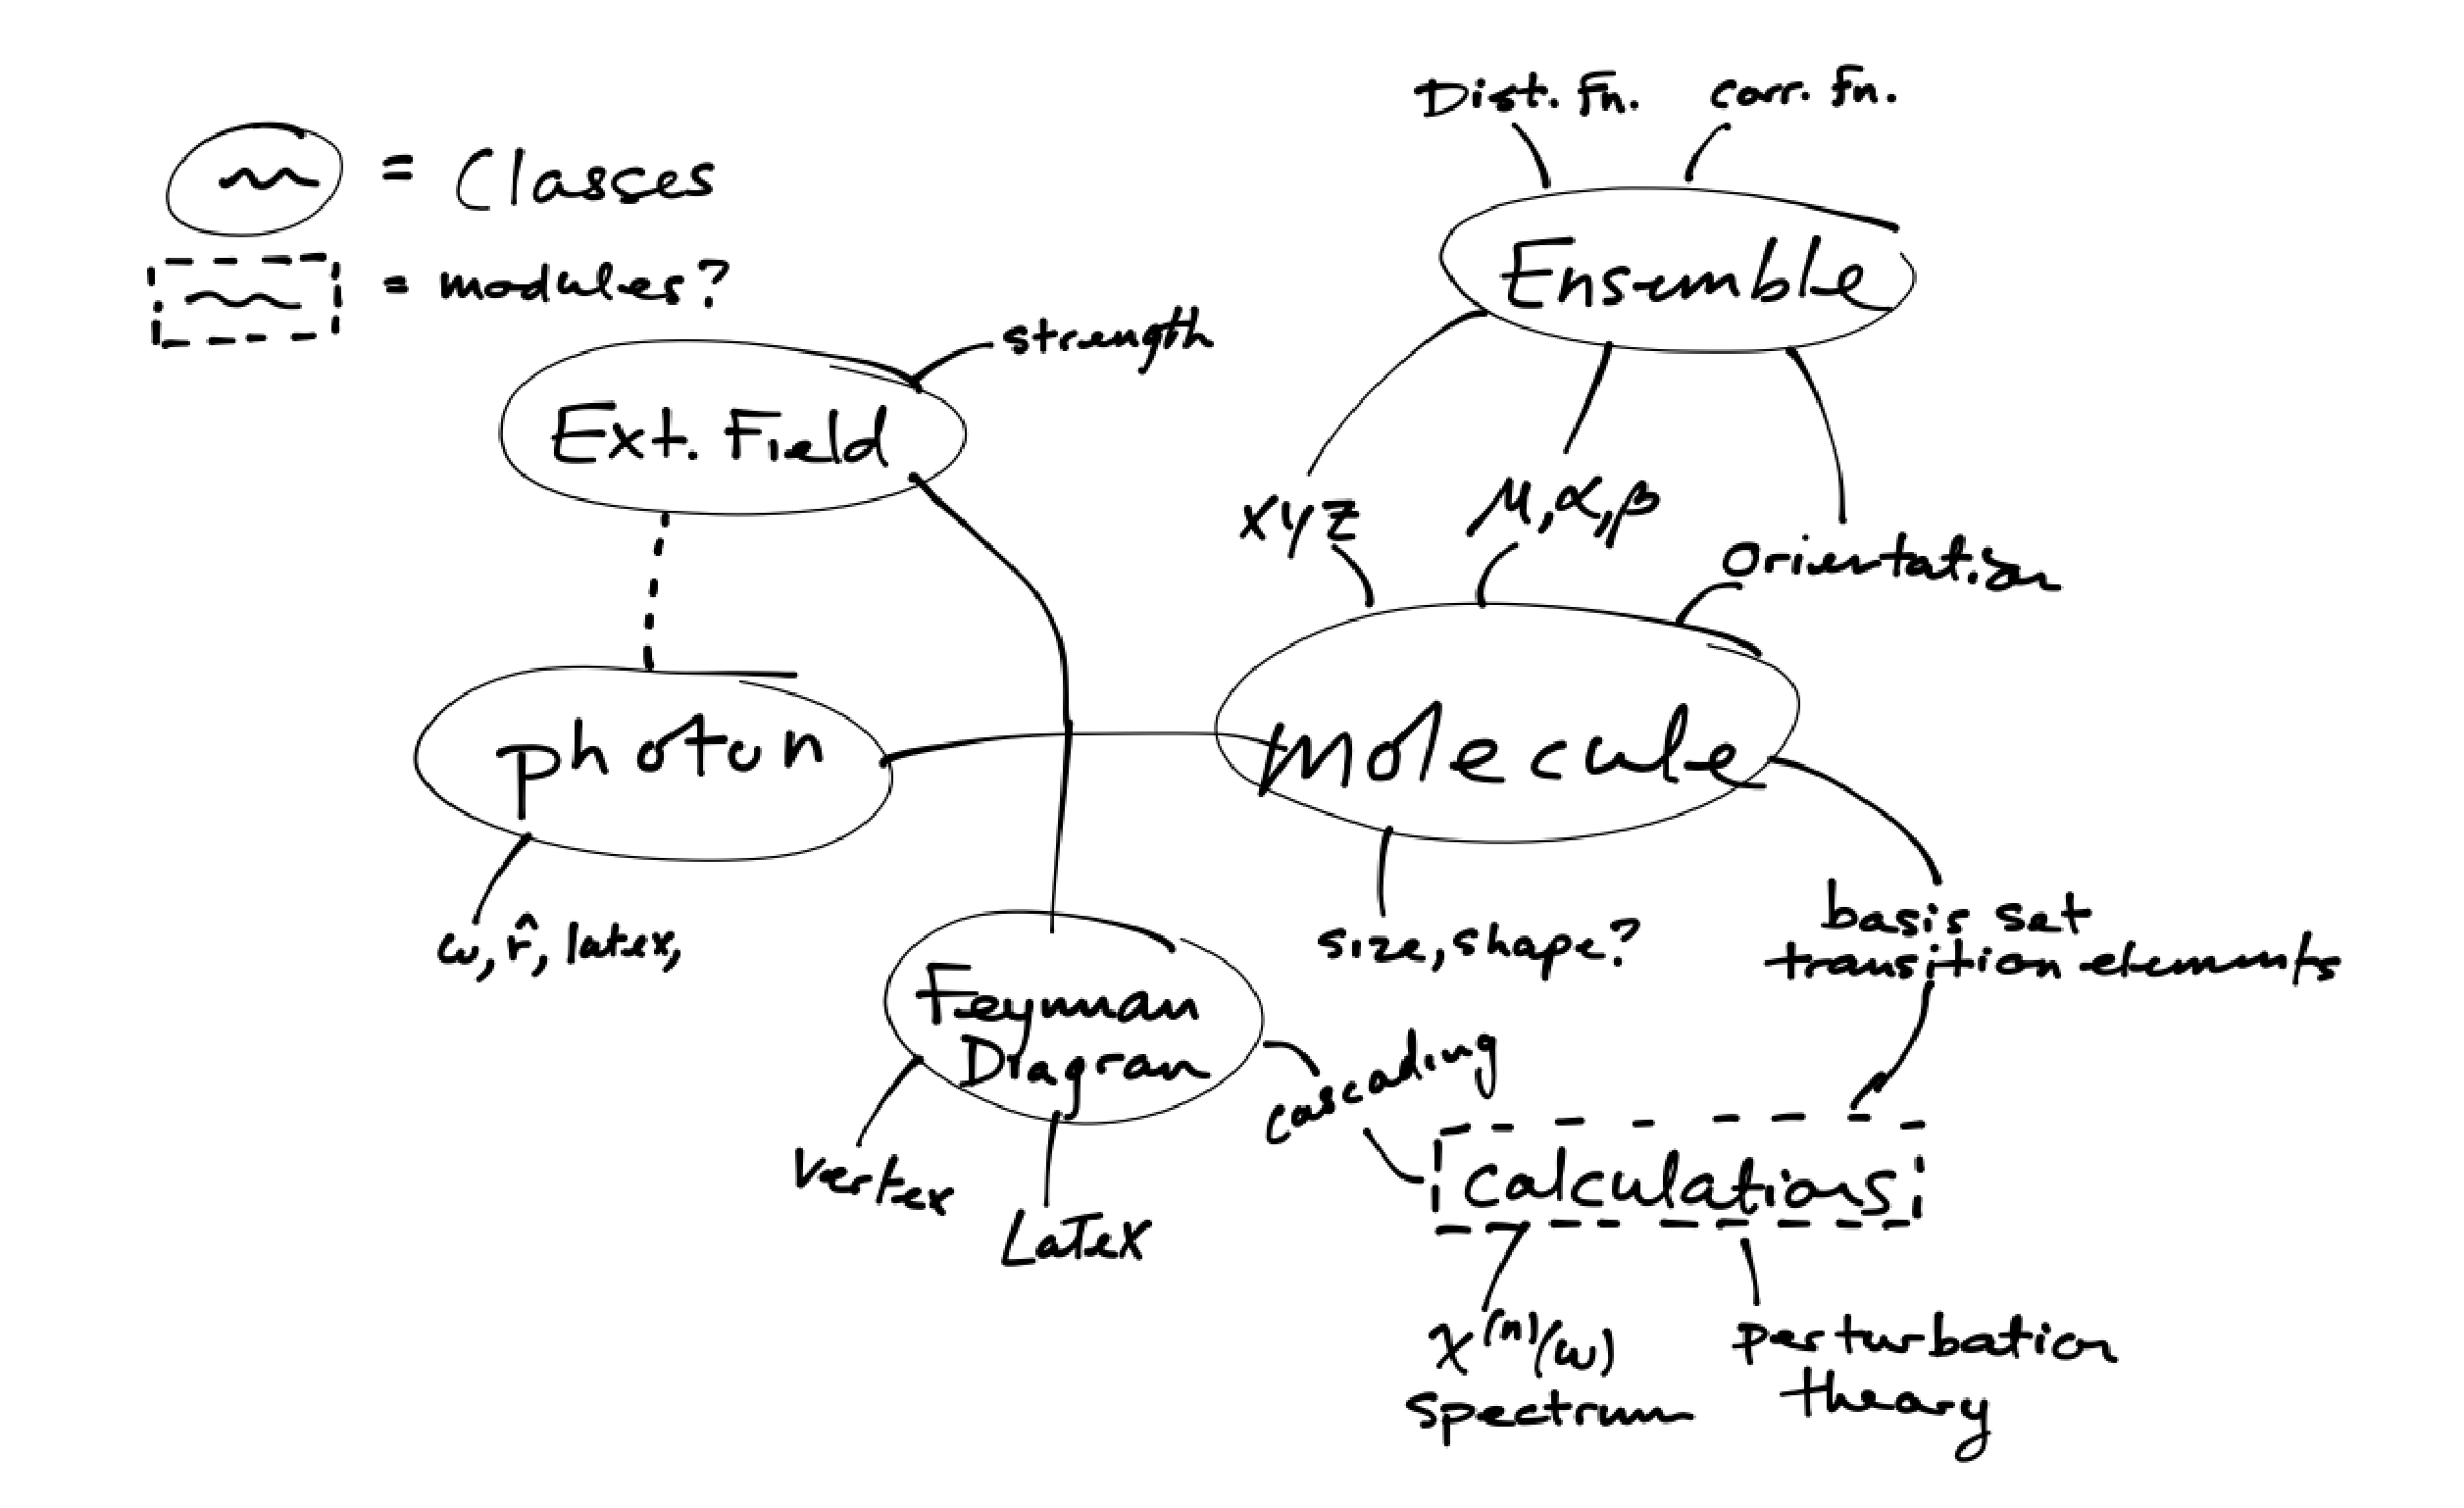
\includegraphics[scale=0.35]{bubblefig.pdf}
\caption{Hypothetical bubble chart indicating possible program structure and implied use relationships.}
\label{fig:bubblechart}
\end{figure}

\section{Getting Started}

As this packages is programmed in Python, Python is required for running any of the following calculations. FeyPy is compatible with Python v2.7 or later. In addition, Numpy 1.8 (or later) and Matplotlib is also required. 

To install FeyPy, simply download and/or extract all source code to a single directory and run with a Python interpreter. At this point, FeyPy is not configured to install directly to your Python path. Expect this to change in later iterations of the code.

The current (pre-alpha) version of FeyPy is v.0.1.

\section{Examples}

The utility of FeyPy is evidenced by its versatility. It is intended to be a one-stop-shop for visualization, calculation and fitting of nonlinear processes to the mind's eye and to experimental data. The following examples should serve as an effective introduction to the basic workings of the code. For questions about specific functions, or for a description of each available function (some are cleverly hidden to avoid accidental malarkey), see the Function Glossary.

\subsection{Constructing a simple Feynman diagram}

Before beginning, be sure that all required packages (outlined in Getting Started) are installed. To import, make the following calls in your interpreter:

\begin{code}
from Feynman import *
from Photon import *
from Permutation import *
from Molecule import *
from CalcChi import *
# eventually, hope to have this simply be replaced with
# from FeyPy import *
import numpy as np
\end{code} 

A Feynman diagram is represented by a Feynman object within FeyPy, or, alternatively, an object of class Feynman. Such an object is defined as follows:

\begin{code}
feyn = Feynman()
\end{code}

In general, there are two types of particles depicted by Feynman diagrams: photons, and molecules that are absorbing or emitting photons. Defining a single Feynman diagram (object) represents the interaction of a single molecule with an arbitrary number of photons. Within FeyPy, photons are treated as objects of the class Photon. In order to define a photon, one needs to input the frequency and polarization as basic information. (Note: Other arguments can be used when defining photons, which will be described later.)

In this example, three photons will be defined.

\begin{code}
photon1 = Photon(1,0)	# the first argument is frequency,
photon2 = Photon(1,0)	# the second argument is polarization
photon3 = Photon(-2,0)
\end{code}

To calculate meaningful results, make sure the output frequency (thus, energy) is the negative sum of the input frequencies. The polarization should be defined as either $0$, $1$, or $2$, representing photons polarized along $x$, $y$, or $z$, respectively. Units are defined such that $\hbar=1$

Once the photons are defined, all that remains is to add the photons to our Feynman diagram by using the \textit{addVertex()} command, which takes individual photon objects as arguments. Implement as follows:

\begin{code}
# for a small number of photons, it might be easier to add individually
feyn.addPhoton(photon1)
feyn.addPhoton(photon2)
feyn.addPhoton(photon3)

# --> OR <-- for a set of photons, it may be easier to add using a for loop
photon_list = [photon1, photon2, ... photonN]
[feyn.addPhoton(photon_list[i]) for i in range(len(photon_list))]
\end{code}

This is the basic information needed to construct a Feynman diagram visualization. See the following sections for visualization methods and other calculations.

\subsection{Viewing a Feynman diagram}

Given the Feynman diagram object \textit{feyn} defined in the previous section, one may visualize the diagram with the following code:

\begin{code}
feyn.showDiagram()
\end{code}

As defined, this call results in the Feynman diagram shown in Fig.~\ref{fig:ex1} (YMMV).

\begin{figure}[h]
\centering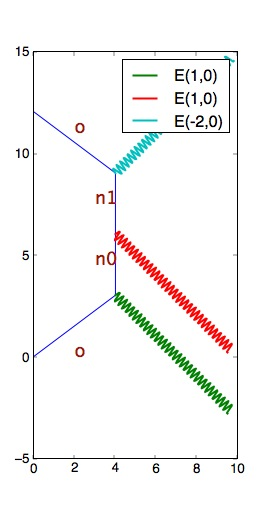
\includegraphics[scale=0.5]{feyn_example1.jpg}
\caption{Example Feynman diagram illustrating a $\chi^{2}$ nonlinear process.}
\label{fig:ex1}
\end{figure}

\subsection{Obtaining $\LaTeX$ code for a Feynman diagram}

In addition to simple visualizations of Feynman diagrams, $\LaTeX$ code corresponding to the equation for the total nonlinear response can be retrieved either as plain text or shown using Matplotlib. In order to return the plain text code, simply use

\begin{code}
feyn.getLaTeX()	# return TeX code as plain text
# returns: '\\chi^{2}=\\sum_{all}\\frac{\\mu^{0}_{gn_1}\\mu^{0}_{n_1n_0}
# \\mu^{0}_{n_0g}}{(\\Omega_{n_{0}g}-\\omega_{1})(\\Omega_{n_{1}g}-2\\omega_{1})}'
\end{code}

which, when copy/pasted into your favorite $\LaTeX$ editor (and with the removal of extra errant backslashes), results in Eq.~\ref{eq:eq_ex1}

\begin{equation}
\chi^{(2)}=\sum_{all}\frac{\mu^{0}_{gn_1}\mu^{0}_{n_1n_0}\mu^{0}_{n_0g}}{(\Omega_{n_{0}g}-\omega_{1})(\Omega_{n_{1}g}-2\omega_{1})}
\label{eq:eq_ex1}
\end{equation}

It is also possible to view Eq.~\ref{eq:eq_ex1} without the use of a $\LaTeX$ compiler using the command

\begin{code}
feyn.showLaTeX()
\end{code}

\subsection{Finding permutations of a Feynman diagram}

The single diagram defined previously is not the whole story. Eq.~\ref{eq:eq_ex1} refers to a sum over potentially many Feynman diagrams, which represent unique permutations of the input/output photons so defined. FeyPy can not only determine what these unique permutations are, but it can also generate Feynman objects for each permutation which can themselves be interacted with using any method defined for Feynman objects. 

To generate these permuted Feynman diagrams, use the following code:

\begin{code}
list_of_feynmans = feyn.getPermutedFeynmans() 
\end{code}

Each element of the defined list is itself a Feynman object, so each can be asked to generate an independent Feynman diagram, as shown in Fig.~\ref{fig:ex1_permutations}.


\begin{figure}[htb]
\centering
\begin{subfigure}{.33\textwidth}
  \centering
  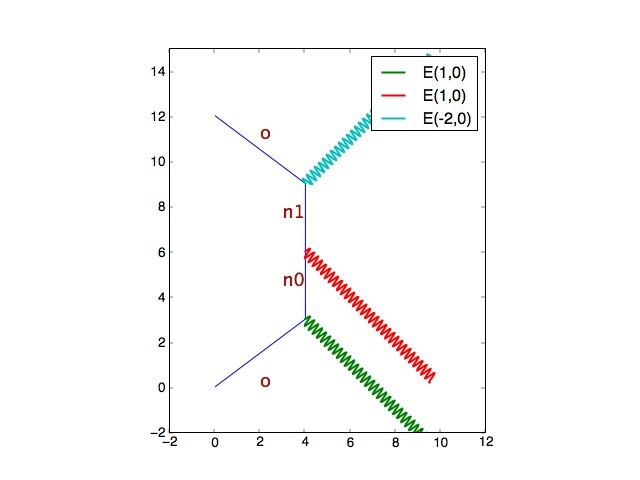
\includegraphics[width=1\linewidth]{feyn_ex1a.jpg}
%  \caption{A subfigure}
  \label{fig:sub1}
\end{subfigure}%
\begin{subfigure}{.33\textwidth}
  \centering
  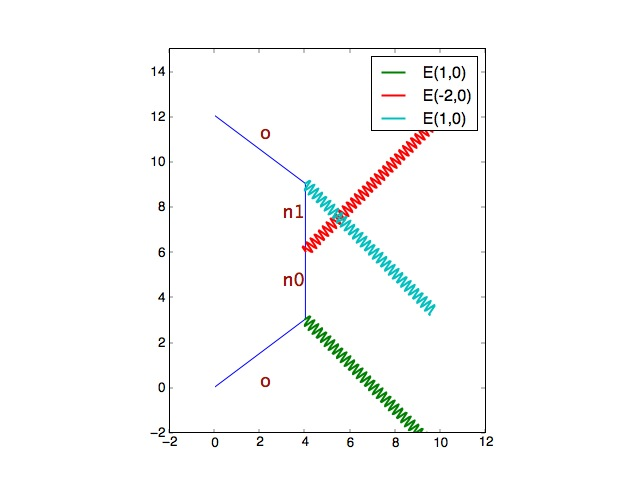
\includegraphics[width=1\linewidth]{feyn_ex1b.jpg}
 % \caption{A subfigure}
  \label{fig:sub2}
\end{subfigure}
\begin{subfigure}{.33\textwidth}
  \centering
  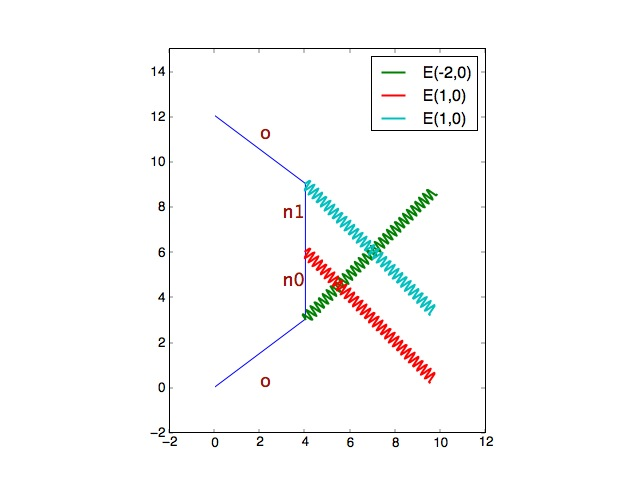
\includegraphics[width=1\linewidth]{feyn_ex1c.jpg}
 % \caption{A subfigure}
  \label{fig:sub3}
\end{subfigure}
\caption{All unique permutations of the example Feynman diagram.}
\label{fig:ex1_permutations}
\end{figure}

\subsection{Calculating the nonlinear response for a single diagram and its permutations}

Beyond the utility of visualizing Feynman diagrams, FeyPy is also capable of calculating nonlinear susceptibilities of individual diagrams or even the total nonlinearity of a set of all possible Feynman diagrams. For the Feynman object already defined as a result of the previous examples, we must first define a set of transition elements (Mu's) and resonant frequencies (Omega's) in order to calculate the nonlinear response. We use the \textit{Molecule} class to achieve this. Objects of class Molecule represent molecules who's interaction with photons are represented by Feynman diagrams (and hence Feynman objects). Besides transition elements, and transition energies, molecule objects also contain position and orientation information relative to the lab frame. This information is necessary for cascading calculations, which will be addressed later. When dealing with single molecules, position and orientation is irrelevant.

\begin{code}
molecule = Molecule()	# make a new molecule

mu = np.array([[[0, 1, 2],	# define mu's
                [1, 2, 3],
                [2, 3, 4]],
               
               [[0, 1, 2],
                [1, 2, 3],
                [2, 3, 4]],
               
               [[0, 1, 2],
                [1, 2, 3],
                [2, 3, 4]]])

molecule.setMu(mu)		# set molecule Mu matrix to mu

molecule.addOmega([1.5,2.5])	# add transition energies
					# to molecule
					# (add either individually, or
					# as a list)

feyn.linkMolecule(molecule)	# link molecule and feyn objects
\end{code}

Now we can calculate the nonlinear response of an individual Feynman object.

\begin{code}
a_chi = feyn.getChi()	# individual response
\end{code}

Or, we can calculate the total nonlinearity for the given system by adding the contributions from each possible Feynman diagram using this function

\begin{code}
a_chi = feyn.getTotalChi()	# from all permutations
\end{code}

%\begin{code}
%total_chi = 0.0	# dummy total variable
%N_diagrams = len(list_of_feynmans)	# total number of possible unique Feynman diagrams
%
%for i in range(N_diagrams):
%	total_chi += list_of_feynmans[i].getChi()
%\end{code}

Another useful feature is the ability to define a photon object as a \textit{spectrum} photon, whereas previously photons were only defined as having a fixed frequency. A spectrum photon as an input into a Feynman diagram allows for the calculation of a spectrum of $\chi$ values, i.e. a $\chi$ vs. $\omega$ plot, for example.

Following the examples laid out previously, but changing the definition of photon1 to the following:

\begin{code}
# defining spectrum frequency photons
photon1 = Photon(1,0,spectrum=True,stepfreq=0.01,startfreq=0.0,endfreq=10.0)
\end{code}

Following the previous steps aside from this minor deviation, the individual (and total) nonlinearity can also be calculated in an analogous way. Note that the \textit{getChi()} method is versatile enough to function with either a spectrum or fixed frequency photon, except that now two results are returned. (Note: Only define a single photon as a spectrum photon.) The results of this calculation are shown in Fig.~\ref{fig:chi_spec}. Currently, there is nothing to prevent the code from inadvertently dividing by zero. This issue needs to be addressed in the future.

\begin{code}
wlist,chi = feyn.getChi()	# wlist, chi, are the spectrum and chi, respectively 
showChiSpectrum(wlist,chi)	# plotting command
\end{code}


\begin{figure}[h]
\centering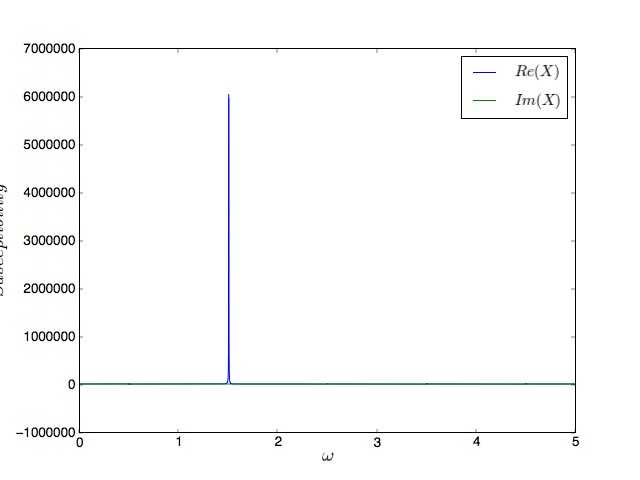
\includegraphics[scale=0.5]{chi_spectrum_fix.jpg}
\caption{Example $\chi^{(2)}$ spectrum for the aforementioned nonlinear process.}
\label{fig:chi_spec}
\end{figure}

The same can be done for the permutations of the Feynman diagram

\begin{code}
wlist,chi = feyn.getTotalChi()	# wlist, chi, are the spectrum and chi, respectively 
showChiSpectrum(wlist,chi)	# plotting command
\end{code}
 which in this case results in the same spectrum as shown in Fig.~\ref{fig:chi_spec}.

\subsection{Cascading between multiple Feynman diagrams}

The bread and butter of FeyPy is its ability to represent nonlinear cascading processes, calculate individual or total nonlinear responses, and return $\LaTeX$ strings corresponding to $\chi^{(n)}$, etc. To cascade two diagrams, a second Feynman object must first be defined, in addition to an object of class Cascade. Both Feynman objects must then be added to the Cascade object, which actually handles cascading processes.

\begin{code}
feyn2 = Feynman()	# new Feynman object
photon4 = Photon(1,0)	# new photons for feyn2
photon5 = Photon(1,0)
photon6 = Photon(-2,0)

feyn2.addPhoton(photon4)	# add new photons to feyn2
feyn2.addPhoton(photon5)
feyn2.addPhoton(photon6)

photon5.toggleVirtual()		# set photon5 to be a virtual

feyn2.linkMolecule(molecule)	# link to first molecule
						# for convenience
\end{code}

Feel free to check the appearance of \textit{feyn2}. It should be appear to be identical to our first Feynman diagram. The two diagrams can be cascaded as follows:

\begin{code}
cascade = Cascade()	# create Cascade object

cascade.addFeynman(feyn)	# add feynman diagrams
cascade.addFeynman(feyn2)	# to cascade

cascade.showDiagram()	# show cascaded diagram
\end{code}

This results in the diagram shown in Fig.~\ref{fig:casc_ex}.

\begin{figure}[h]
\centering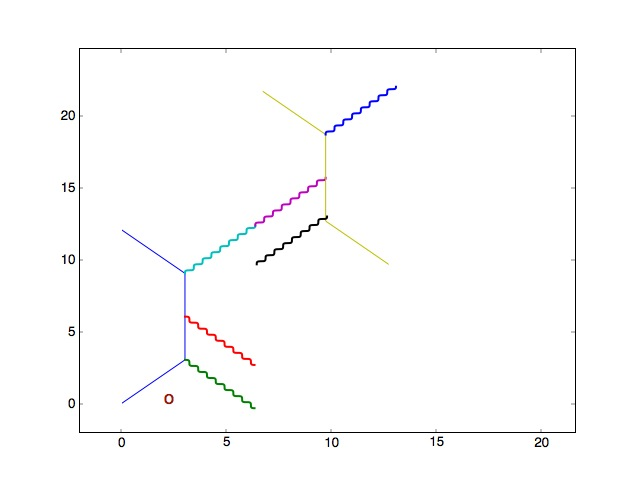
\includegraphics[scale=0.5]{cascading_ex4.jpg}
\caption{Example of a cascading process.}
\label{fig:casc_ex}
\end{figure}

\pagebreak

\section{Code Glossary}

\subsection{Test Script}

\begin{code}
import Feynman
import Photon
import Mu
import Omega
import CalcChi
import Permutation
import Molecule
import Cascade
import numpy as np

feyn = Feynman.Feynman()

useFixed = False #set to false for fixed frequency photons


if(useFixed is True):
    # testing fixed frequency photons
    photon1 = Photon.Photon(1,0)
    photon2 = Photon.Photon(1,0)
    photon3 = Photon.Photon(-2,0)

else:
    # testing spectrum frequency photons
    photon1 = Photon.Photon(1,0,spectrum=True,stepfreq=0.001,startfreq=0.0,endfreq=5.0)
    photon2 = Photon.Photon(1,0)
    photon3 = Photon.Photon(-2,0)


# make a molecule!
molecule = Molecule.Molecule()

# define mu's
mu = np.array([[[0, 1, 2],
                [1, 2, 3],
                [2, 3, 4]],
               
               [[0, 1, 2],
                [1, 2, 3],
                [2, 3, 4]],
               
               [[0, 1, 2],
                [1, 2, 3],
                [2, 3, 4]]])

# add Mu matrix to molecule
molecule.setMu(mu)

# add omega's to molecule
molecule.addOmega([1.5,2.5])

# link molecule to Feynman object
feyn.linkMolecule(molecule)

# add vertices to diagram
feyn.addPhoton(photon1)
feyn.addPhoton(photon2)
feyn.addPhoton(photon3)

# show feynman diagram
#feyn.showDiagram()

# check out the latex code!
# we can either render it on a figure:
#feyn.showLaTeX()

# or we can return it as a string for easy copying into TeX editors
#feyn.getLaTeX()

# getChi!
#if(useFixed is True):
#    chi = feyn.getChi()
#    print(chi)
#
#else:
#    a = feyn.getChi()
#CalcChi.showChiSpectrum(wlist,chi)


# test out permutations
# returns a set of feynman diagrams with photon frequency,polarization
# tuples permuted according to Kyle's permutations code
list_of_feynmans = feyn.getPermutedFeynmans()

# make phton3 virtual
photon3.toggleVirtual()

# make some more photons
photon4 = Photon.Photon(1,0)
photon5 = Photon.Photon(1,0)
photon6 = Photon.Photon(-2,0)

photon5.toggleVirtual()

next_feyn = Feynman.Feynman()
next_feyn.addPhoton(photon4)
next_feyn.addPhoton(photon5)
next_feyn.addPhoton(photon6)
next_feyn.linkMolecule(molecule)

# make a cascade object
cascade = Cascade.Cascade()

# add feynman objects to cascade
cascade.addFeynman(feyn)
cascade.addFeynman(next_feyn)

# show cascaded diagram
cascade.showDiagram()
\end{code}

\subsection{Class: Feynman}

\begin{code}
#Import Modules/CLasses
import Photon
import CalcChi
import Permutation
import Diagram
import LaTeX
import itertools

#Import Libraries
import matplotlib.pyplot as plt
import numpy as np

class Feynman(object):
    
    def __init__(self):
        self.photon_list = []
        self.linkedMol = None
        self.latex_string = ''
    
    def linkMolecule(self,molecule):
        self.linkedMol = molecule
    
    def getLinkedMolecule(self):
        return self.linkedMol

    def getChi(self):
        # use this method expressly to get nonlinearity for single diagram for either
        # spectrum or specific set of frequencies
        freq_list  = self.getTupleSet()
        mu_list    = self.getLinkedMolecule().getMu()
        Omega_list = self.getLinkedMolecule().getOmegas()
        photons = self.getPhotonList()
        
        # are there any "spectrum" photons? if so, need to use calcChiSpectrum()
        # else, for only fixed photons, use calcChi()
        # FIRST: Check for spectrum photons!
        
        num_spectrum_photons = 0
        spectrum_photon_index = []
        
        for p in range(len(photons)):
            if (photons[p].isSpectrum() is True):
                # found a spectrum photon, save it's index
                num_spectrum_photons += 1
                spectrum_photon_index.append(p)
        
        
        # SECOND: If no spectrum photons, get single valued Chi
        
        if(num_spectrum_photons==0):
            return CalcChi.calcChi(freq_list, mu_list, Omega_list)
        
        # THIRD: If only one spectrum photon, get Chi spectrum
        
        elif(num_spectrum_photons==1):
            freq_spectrum = photons[spectrum_photon_index[0]].getSpectrum()
            wlist,chi = CalcChi.calcTotalChiSpectrum(spectrum_photon_index[0],freq_spectrum,mu_list,Omega_list,freq_list)
            return wlist,chi
        
        # FOURTH: If more than one spectrum photon, return 0 (for now)
        
        else:
            # This will return data to make a 3D plot (featuring a 2D chi surface)
            return 0

    def getTotalChi(self):
        # use this method expressly to get total nonlinearity for either
        # spectrum or specific set of frequencies
        freq_list  = self.getTupleSet()
        mu_list    = self.getLinkedMolecule().getMu()
        Omega_list = self.getLinkedMolecule().getOmegas()
        photons = self.getPhotonList()
        
        # are there any "spectrum" photons? if so, need to use calcChiSpectrum()
        # else, for only fixed photons, use calcChi()
        # FIRST: Check for spectrum photons!
        
        num_spectrum_photons = 0
        spectrum_photon_index = []
        
        for p in range(len(photons)):
            if (photons[p].isSpectrum() is True):
                # found a spectrum photon, save it's index
                num_spectrum_photons += 1
                spectrum_photon_index.append(p)
        
        
        # SECOND: If no spectrum photons, get single valued Chi
        
        if(num_spectrum_photons==0):
            return CalcChi.calcChiPermutations(freq_list, mu_list, Omega_list)
        
        # THIRD: If only one spectrum photon, get Chi spectrum
        
        elif(num_spectrum_photons==1):
            freq_spectrum = photons[spectrum_photon_index[0]].getSpectrum()
            wlist,chi = CalcChi.calcTotalChiSpectrum(spectrum_photon_index[0],freq_spectrum,mu_list,Omega_list,freq_list)
            return wlist,chi
        
        # FOURTH: If more than one spectrum photon, return 0 (for now)
        
        else:
            # This will return data to make a 3D plot (featuring a 2D chi surface)
            return 0
    
    def getLaTeX(self):
        self.updateLaTeX()
        return self.latex_string
    
    def showLaTeX(self):
        self.updateLaTeX()
        plt.text(0.5,0.5,'$%s$'%self.latex_string)

    def updateLaTeX(self):
        freq_list = self.getTupleSet()  #list of frequency,polarization tuples
        chi_string = LaTeX.latex(freq_list)
        self.latex_string = chi_string
    
    def showDiagram(self):
        freq_list = self.getTupleSet()
        Diagram.diagram(freq_list)
    
    def addPhoton(self,photon):
        self.photon_list.append(photon)

    def getPhotonList(self):
        return self.photon_list

    def getPermutedFeynmans(self):
        # This method finds all possible permutaions of a list of photon
        # objects, returns a list of Feynman objects, each with a different
        # possible permutation
        
        feyn_list = []  #list of feynman diagrams
        photon_list = self.getTupleSet()
        N_photons = len(photon_list)

        permuted_photons = Permutation.getPermutations(photon_list)
        N_permutations = len(permuted_photons)

        # create list of feynman objects for each permutation
        for i in range(N_permutations):
            temp_feyn = Feynman()   #new feynman diagram
            for j in range(N_photons):
                # generate temp_photon from permutation
                temp_tuple = permuted_photons[i][j]
                temp_photon = Photon.Photon(temp_tuple[0],temp_tuple[1])
                #add new photon to new feynman diagram
                temp_feyn.addPhoton(temp_photon)
            
            # make Omegas and Mus consistent for all permutations of feyn
            temp_feyn.linkMolecule(self.linkedMol)
            
            # add new feynman diagram to list of feynman diagrams
            feyn_list.append(temp_feyn)

        return feyn_list

    def getTupleSet(self):
        # This method generates a list of tuples from self.photon_list
        
        tuple_set = []
        photons = self.getPhotonList()
        N_photons = len(photons)
        
        for i in range(N_photons):
            tuple_set.append(photons[i].getTuple())
        
        return tuple_set

\end{code}

\subsection{Class: Photon}

\begin{code}
import matplotlib.pyplot as plt
from math import ceil,sqrt
import numpy as np

class Photon(object):
    
    def __init__(self,frequency,polarization,**kwargs):
        self.tuple = [frequency,polarization]
        self.virtual = False
        self.spectrum = False
        self.dw = None
        self.start_freq = None
        self.end_freq = None
    
        # check if photon is spectrum photon!
        # can add other conditional arguments here as necessary
        for k,v in kwargs.iteritems():
            if(k=="spectrum" and v==True):
                self.spectrum = v
            elif(k=="stepfreq"):
                self.dw = v
            elif(k=="startfreq"):
                self.start_freq = v
            elif(k=="endfreq"):
                self.end_freq = v
    
        if (self.spectrum==True):
            Npoints = int(ceil(float(self.end_freq - self.start_freq)/float(self.dw)))
            self.freq_spectrum = [ i*self.dw for i in range(Npoints) ]
    
    def getTuple(self):
        return self.tuple

    def setTuple(self,new_tuple):
        self.tuple = new_tuple

    def isVirtual(self):
        return self.virtual

    def toggleVirtual(self):
        # if virtual == true, set to false
        # if virtual == false, set to true
        self.virtual = not self.virtual

    def isSpectrum(self):
        return self.spectrum

    def getSpectrum(self):
        return self.freq_spectrum

    def setSpectrum(self,start,end,dw):
        Npoints = int(ceil(float(end - start)/float(dw)))
        self.freq_spectrum = [ start+i*dw for i in range(Npoints) ]

    def toggleSpectrum(self):
        # if spectrum == true, set to false
        # if spectrum == false, set to true
        self.spectrum = not self.spectrum

    def isMatch(self,photon):
        my_tuple = self.getTuple()
        test_tuple = photon.getTuple()
    
        if (my_tuple==test_tuple):
            return True
        else:
            return False


\end{code}

\subsection{Class: Molecule}

\begin{code}
import numpy as np

class Molecule(object):
    
    def __init__(self):
        self.orientation = np.array([0.0,0.0,0.0])
        self.position = np.array([0.0,0.0,0.0])
        self.mu = []
        self.Omega_list = []
    
    def setPosition(self,x,y,z):
        self.position = np.array([x,y,z],dtype=float)
    
    def getPosition(self):
        return self.position
    
    def setOrientation(self,rho,theta,phi):
        self.orientation = np.array([rho,theta,phi],dtype=float)
    
    def getOrientation(self):
        return self.orientation
    
    def setMu(self,new_mu):
        self.mu = np.array(new_mu,dtype=float)
    
    def getMu(self):
        return self.mu
    
    def addOmega(self,new_Omegas):
        new_Omegas = np.array(new_Omegas,dtype=float).flatten()
        [self.Omega_list.append(new_Omegas[i]) for i in range(len(new_Omegas))]

    def getOmegas(self):
        return np.array(self.Omega_list,dtype=float)\end{code}

\subsection{Class: Cascade}

\begin{code}
import matplotlib.pyplot as plt
from math import ceil,sqrt
import numpy as np
import Diagram

class Cascade(object):
    
    def __init__(self):
        self.list_of_feynmans = []
        self.latex_string = ''
    
    def addFeynman(self,feyn):
        self.list_of_feynmans.append(feyn)
    
    def getFeynmanList(self):
        return self.list_of_feynmans

    def showDiagram(self):
        tuple_sets = []
        N_feynmans = len(self.list_of_feynmans)
        photon_lists = []
        vert_num = 0
        
        for i in range(N_feynmans):
            temp_photon_list = self.list_of_feynmans[i].getPhotonList()
            temp_tuple_set = self.list_of_feynmans[i].getTupleSet()
            photon_lists.append(temp_photon_list)
            tuple_sets.append(temp_tuple_set)
            
            for j in range(len(temp_photon_list)):
                if(temp_photon_list[j].isVirtual()):
                    tuple_sets[i][j][1] = 3
    
        if(N_feynmans==2):
            for i in range(len(photon_lists[-1])):
                if(photon_lists[-1][i].isVirtual()):
                    vert_num = i
        
#        return tuple_sets,vert_num,photon_lists

        Diagram.chain_diagram(tuple_sets[0],tuple_sets[1],0,vert_num)

    def getPermutations(self):
        return 0

    def getLaTeX(self):
        # to be written
        return 0
    
    def showLaTeX(self):
        # to be written
        return 0
\end{code}

\subsection{Module: LaTeX}

\begin{code}
def latex(photons):
    """Generates some latex code that shows chi^n all nice and pretty
    Input:
        photons == the photons interacting with the system in the order
        they interact with the system
    Output:
        chi == this is the python version of latex used to make a pic of the
        equation.
        
    How to use:
        ~make an array of your incoming photons! It should look like this:
        myphotons = [[frequency, polarization],[frequency,polarization],...]
        ~run the code like this:
        latex(myphotons)
        ~wait impatiently.
    """
    
    import pylab as py
    import numpy as np
    import matplotlib.pyplot as plt
    
    photons = np.array(photons) #changing the input to np arrays
    
    #Find how many photons we be using.
    N = len(photons)
    #Initialize the output strings
    energy = ''
    #energytex=''
    mu = ''
    chi=''
    #chitex=''
    #mutex= '' #saving this in case we want to be able to copy and paste the latex output code and not have the extra \
    w = 0

  #The following for loop figures out the numerator. Since we don't
  #need to worry about complex conjugates, it is a pretty easy loop.  
    for i in xrange(N):
        if i==0: #making sure the mu starts at the ground level, g
            mu ='\\mu^{'+str(photons[i,1])+'}_{n_0g}'
            #mutex ='\mu^{'+str(photons[i,1])+'}_{n_0g}'
        elif i==N-1: #this is the last photon. Make sure mu goes back to ground level
            mu ='\\mu^{'+str(photons[i,1])+'}_{gn_'+str(i-1)+'}'+mu
            #mutex ='\mu^{'+str(photons[i,1])+'}_{gn_'+str(i-1)+'}'+mutex
        else: #besides the first and last photon, the rest don't need special treatment
            mu ='\\mu^{'+str(photons[i,1])+'}_{n_'+str(i)+'n_'+str(i-1)+'}'+mu
            #mutex ='\mu^{'+str(photons[i,1])+'}_{n_'+str(i)+'n_'+str(i-1)+'}'+mutex
            
    #The following section makes the energy denominator. It is more complicated. :/
    
    freq = np.zeros(N)
    #freq just records the frequency of each photon in the order they came in
    for i in xrange(N):
        freq[i]=photons[i,0]
        
    #a just catches the output from the checker function below. coeff and uniques
    #are then the actual output of the checker. I could skip the 'a' but I'm stupid
    #and don't know how
    a=checker(freq)
    coeff=a[0]
    uniques=a[1]

    #actual loop making the energy denominator. i goes from zero to one less than
    #the number of photons you sent in.
    for i in xrange(N-1):
        w += photons[i,0] #sum of all the incoming and outgoing photons
        if w>=0: #if the photons are all coming in (or the total is zero), no complex conjugate is needed!
            energy = energy +'(\\Omega_{n_{'+str(i)+'}g}' #this line starts the energy denominator
            #energytex= energytex +'(\Omega_{n_{'+str(i)+'}g}'
            for n in xrange(len(uniques)+1):
                if coeff[i,n]==0 or n==len(uniques)+1: #this tells the loop to close the bracket
                    energy= energy +')'
                    #energytex=energytex+')'
                    break
                elif coeff[i,n]==1: #we don't need 1*w, we just want w
                    if uniques[n]<0: #outgoing photon! better add it!
                        energy = energy + '+\\omega_{'+str(-1*int(uniques[n]))+'}'
                   #     energytex = energytex + '+\omega_{'+str(-1*int(uniques[n]))+'}'
                    elif uniques[n]>0: #incoming photon! SUBTRACT! SUBTRACT!
                        energy = energy + '-\\omega_{'+str(int(uniques[n]))+'}'
                  #      energytex = energytex + '-\omega_{'+str(int(uniques[n]))+'}'
                    else: #that's boring. you sent in a photon of zero frequency
                        1
                else: #here is where the non-1 coefficients come in
                    if uniques[n]<0: #outgoing photon! better add it!
                        energy = energy + '+' +str(int(coeff[i,n]))+'\\omega_{'+str(-1*int(uniques[n]))+'}'
                 #       energytex = energytex + '+' +str(int(coeff[i,n]))+'\omega_{'+str(-1*int(uniques[n]))+'}'
                    elif uniques[n]>0: #incoming photon! SUBTRACT! SUBTRACT!
                        energy = energy + '-' +str(int(coeff[i,n]))+'\\omega_{'+str(int(uniques[n]))+'}'
                #        energytex = energytex + '-' +str(int(coeff[i,n]))+'\omega_{'+str(int(uniques[n]))+'}'
                    else: #that's boring. you sent in a photon of zero frequency
                        1
        elif w<0: #ohgodohgodohgod energy is negative! help me!
            energy = energy +'(\\Omega_{n_'+str(i)+'g}^*' #complex conjugate that shit
            #energytex = energytex +'(\Omega_{n_'+str(i)+'g}^*'
            for n in xrange(len(uniques)+1):
                if coeff[i,n]==0 or n==len(uniques)+1: #see above
                    energy= energy +')'
                    #energytex= energytex +')'
                    break
                elif coeff[i,n]==1:
                    if uniques[n]<0: #outgoing photon! better add it!
                        energy = energy + '+\\omega_{'+str(-1*int(uniques[n]))+'}'
                        #energytex = energytex + '+\omega_{'+str(-1*int(uniques[n]))+'}'
                    elif uniques[n]>0: #incoming photon! SUBTRACT! SUBTRACT!
                        energy = energy + '-\\omega_{'+str(int(uniques[n]))+'}'
                        #energytex = energytex + '-\omega_{'+str(int(uniques[n]))+'}'
                    else: #that's boring. you sent in a photon of zero frequency
                        1
                else:
                    if uniques[n]<0: #outgoing photon! better add it!
                        energy = energy + '+' +str(int(coeff[i,n]))+'\\omega_{'+str(-1*int(uniques[n]))+'}'
                        #energytex = energytex + '+' +str(int(coeff[i,n]))+'\omega_{'+str(-1*int(uniques[n]))+'}'
                    elif uniques[n]>0: #incoming photon! SUBTRACT! SUBTRACT!
                        energy = energy + '-' +str(int(coeff[i,n]))+'\\omega_{'+str(int(uniques[n]))+'}'
                        #energytex = energytex + '-' +str(int(coeff[i,n]))+'\omega_{'+str(int(uniques[n]))+'}'
                    else: #that's boring. you sent in a photon of zero frequency
                        1                
        else:
            1 #do nothing.
            
    chi= '\\chi^{('+str(N-1)+')}=\sum_{all}\\frac{'+mu+'}{'+energy+'}'
                                    
# plt.plot;plt.text(0.5,0.5,'$%s$'%chi,fontsize=15)
#   plt.show()
    
    return chi
    
def checker(photons):
    """The energy denominator can't have terms like E-hw1-hw1 because it should
    be E-2hw1. This function determines the coefficient in front of the
    input frequency (w1 in the example).
    Input:
        photons == the photons interacting with the system in the order
        they interact with the system, frequency only!
    Output:
        m == a matrix of size mXn where m is the number of incoming photons
        and n is the number of UNIQUE incoming photons. This matrix contains
        coefficients for calculating the energy denominator
        
        temp == a vector of the unique photons in your system
        
    How to use:
        ~make an array of your incoming photons! It should look like this:
        myphotons = [frequency1, frequency2, ...] (NO POLARIZATION!)
        ~run the code like this:
        checker(myphotons)
        ~wait impatiently.
    """
    import numpy as np
    
    N=len(photons)
    temp=list(photons)
    photons = list(photons) #changing the input to a list
    
    
    #this loop goes through the temporary array and keeps the unique items.
    for i in xrange(len(temp)):
        j=i+1
        while j <len(temp):
            if temp[i] == temp[j]:
                del temp[j]
            else:
                j=j+1
                
    m=np.zeros(shape=(N,len(temp))) #making a matrix
    
    i=0 #prolly don't need to reset these, but just in case...
    j=0
    
    
    #now, compare the unique items to the original input.
    #i is rows. this is equal to the number of incoming photons
    #j is columns. this is equal to the number of unique incoming photons.
    #m is a matrix that contains the coefficients that need to be in front of
    #the omegas.

    for i in xrange(N):
        w = photons[:i+1]
        for j in xrange(len(temp)):
            m[i,j]=w.count(temp[j])
            
    m = np.array(m) #I've been messing with strings here. this turns them
    temp = np.array(temp) #back in to numpy arrays so the main latex function can deal with them.
                
    return(m,temp)
\end{code}

\subsection{Module: CalcChi}

\begin{code}
import numpy as np
import math
import matplotlib.pyplot as plt
from Permutation import getPermutations


def calcChi(w, mu, Omega):
    """Calculates the sum over states contribution to the appropriate 
    nonlinearity for the collection of input and output photon frequencies, w,
    the electronic system defined by the transition moments mu and the energy
    levels Omega."""

    
    #Make sure the inputs were entered as numpy arrays
    w = np.array(w,dtype=float)         #Phton info, freq n polariz
    mu = np.array(mu,dtype=float)       #dipole transition moments
    Omega = np.array(Omega,dtype=float) #Energy diff
    
    
    #Constants
    hbar = 1               #hbar
    N  = len(w) - 1        #Photon - 1, nonlinearity
    NumStates = len(mu[0]) #Number of electronic states
    omegasigma = float(w[0,0])    #To begin with
    
    
    
    #Physics Check for consistancy between transitions and energies
    if NumStates != len(Omega)+1:
        print('Err: Inconsistant electronic state information.')
        return 0



    #Determine vector term for first vertex
    if omegasigma >= 0:
        xi = mu[w[0,1], 1:, 0]/(Omega - omegasigma)
    else:
        xi = mu[w[0,1], 1:, 0]/(Omega.conjugate() - omegasigma)
    
    #Dot in from the left each additional propogator matrix
    for i in np.arange(1, N):
        omegasigma += w[i,0]
        prop = np.array(mu[w[i,1],1:,1:] - mu[w[i,1],0,0])
        if omegasigma > 0:
            prop = np.transpose(np.divide(np.transpose(prop),(Omega - omegasigma)))
        else:
            prop = np.transpose(np.divide(np.transpose(prop),(Omega.conjugate() - omegasigma)))
        xi = np.dot(prop, xi)

    #Dot in the last transition, back to the ground state
    xi = np.dot(mu[w[-1,1],0,1:],xi)
    xi = xi / hbar**N
    
    return xi

#def calcChiSpectrum(F,w1,w2,dw,mu,Omega,w):
def calcChiSpectrum(F,freq_list,mu,Omega,w):
    """Graphs Chi varrying only the Fth w, aka w[F]
        
        F  = Fth fixed photon
        freq_list = a list of photons from w1 to w2 in increments of dw"""
    
    w = np.array(w,dtype=float) #Phton info, freq n polariz
    mu = np.array(mu,dtype=float) #dipole transition moments
    Omega = np.array(Omega,dtype=float) #Energy diff
    wlist = np.array(freq_list,dtype=float) # frequency spectrum
   
    N = len(wlist) #number of freq
    Chi = np.zeros(N) #list to store the Chi of each freq

    #Old Code
    #N     = int(math.ceil(float(w2-w1)/float(dw)))
    #wlist = [w1+i*dw for i in range(N)]
    
    
    
    #Calc X for each w
    for i in range(N):
        w[F]   = [wlist[i],w[F,1]]
        #w[F,0]  = wlist[i]
        Chi[i]  = calcChi(w,mu,Omega)
    
    return wlist,Chi

def calcTotalChiSpectrum(F,freq_list,mu,Omega,w):
    """Graphs Chi varrying only the Fth w, aka w[F]
        
        F  = Fth fixed photon
        freq_list = a list of photons from w1 to w2 in increments of dw"""
    
    w = np.array(w,dtype=float) #Photon info, freq n polariz
    mu = np.array(mu,dtype=float) #dipole transition moments
    Omega = np.array(Omega,dtype=float) #Energy diff
    wlist = np.array(freq_list,dtype=float) # frequency spectrum
    
    N = len(wlist) #number of freq
    Chi = np.zeros(N) #list to store the Chi of each freq
    
    #Old Code
    #N     = int(math.ceil(float(w2-w1)/float(dw)))
    #wlist = [w1+i*dw for i in range(N)]
    
    
    #Calc X for each w
    for i in range(N):
        w[F]   = [wlist[i],w[F,1]]
        #w[F,0]  = wlist[i]
        Chi[i]  = calcChiPermutations(w,mu,Omega)
    
    return wlist,Chi


def showChiSpectrum(wlist,Chi):

    #Graphing
    ReChi    = Chi.real                #Re[Chi]
    ImChi    = Chi.imag                #Im[Chi]

    plt.plot(wlist,ReChi,label = r'$Re(X)$')
    plt.plot(wlist,ImChi,label = r'$Im(X)$')
    plt.xlabel(r'$\omega$',fontsize=17)
    plt.ylabel(r'$Susceptibility$',fontsize=17)
    plt.legend(loc='upper right')
    plt.show()

def calcChiPermutations(w, mu, Omega):
    
    w = np.array(w,dtype=float)       #Phton info, freq n polariz
    mu = np.array(mu,dtype=float)      #dipole transition moments
    Omega = np.array(Omega,dtype=float)   #Energy diff
    permutearray = getPermutations(w) #permutations of w
    chi = 0.0
    
    for i in range(len(permutearray)):
        chi += calcChi(permutearray[i], mu, Omega)
    
    return chi


\end{code}

\subsection{Module: Permutation}

\begin{code}
############################################################
#Programmer: Kyle Schademan,Ted Delikatny, and Adam Goler
# 
#Created: 16 April, 2014 Most recent update:  9 May 2014 (Goler)
# 
#Program description: Permutation program 
############################################################ 
  
import numpy as np 
import math 
import pylab as py
import itertools as it
  

def permute(Warrray):
    """ Converts the list of photons into a numbered list in which similar photons have the same lable. ex [1,1,2,5,2] -> [0,0,2,3,2] """
    uniW = [i for i in range(len(Warrray))]
    for i in range(0,len(Warrray)):
        for j in range(i+1,len(Warrray)):
            if(np.array_equal(Warrray[i],Warrray[j])):
                uniW[j] = uniW[i]
    return uniW

def unique(iterable):
    """Eliminates duplicates from a list """
    seen = set()
    for x in iterable:
        if x in seen:
            continue
        seen.add(x)
        yield x


def getPermutations(Warray):
    """ Records all possible unique permutations of w in an array """
    permutearray = []
    for a in unique(it.permutations(permute(Warray))):
        urple = [Warray[x] for x in a]
        permutearray.append(urple)

    
    return np.array(permutearray)


def permutations_array (array):
    """ 
    inputs: 
        array = two dimensional array 
    outputs: 
        permutations = an array containing all the permutation  
            arrays of the input array 
    """
    # initialize variables 
    unique = 0 
    myorder = [i for i in range(0,len(array))] 
    order = [] 
    temp1 = 0
    temp2 = 0
    temp3 = 0
    index = 0  
    check = 0 
    m = 0
    n = 0
    elements = []  
    integer_order = [] 
              
    # find the number of unique elements in the input array 
    # and create an array to label their locations in the array
    for i in range(0, len(array)): 
          
        for j in range(i+1, len(array)): 
              
            if(np.array_equal(array[i],array[j])): 
                check = 1
              
        if(check == 0): 
            unique = unique +1
            order = py.append(order, i) 
        check = 0
      
    # change elements in order into integers because python
    #needs me to tell it to do this.
    for n in order: 
        integer_order.append(int(n)) 
    order = integer_order 
      
    #put the unique elements of array in an array 
    elements = [array[i] for i in order]
    
    #create an array to count the number of times an element 
    #occurs in the input array 
    degen = [0 for i in range(unique)] 
      
    # find the number of degeneracies of each element of array 
    for k in range(0, len(degen)): 
              
        for j in range(0, len(array)): 
                      
            if(np.array_equal(elements[k],array[j])): 
                degen[k] = degen[k] +1
        
    # find the k-permutation number  
    kpermutation = math.factorial(len(array))              
    for i in range(len(degen)):             
        kpermutation = kpermutation/math.factorial(degen[i]) 
      
    #construct an output array of the corret size 
    permutations = [array for i in range (kpermutation)] 
      
    # permute all of the rotation permutations 
    while(True): 
          
        index = index + 1
        temp1 = myorder[0] 
          
        for i in range(0,len(array)): 
              
            if(i+1<len(array)):         
                myorder[i] = myorder[i+1] 
            else: 
                myorder[i] = temp1 
    
        if(index >= len(permutations)): 
            break  
                      
        permutations[index] = [permutations[index][j] for j in myorder] 
  
  
    # permute the swapping permutations 
    if (unique > 1): 
          
        m = 0
        n = 1
        index = 0
        temp3 = len(array) - 1
          
        while(True): 
                   
            #checks if every element in permutations is unique 
            check = 0                
            for j in range(0, len(permutations)): 
                      
                if(j != temp3): 
                          
                    if(np.array_equal(permutations[temp3],permutations[j])): 
                        check = 1
              
            if(check == 0): 
                temp3 = temp3+1
                index = 0
            else: 
                  
                if(m == len(array)- 1): 
                    m = m-len(array)-1
                else: 
                    m = m+1
                if(n == len(array)-1): 
                    n = n-len(array)-1
                else: 
                    n = n+1
              
            #ends loop if every element is unique 
            if(temp3 == len(permutations)): 
                break
                  
            temp1 = myorder[m] 
            temp2 = myorder[n] 
            myorder[m] = temp2 
            myorder[n] = temp1 
              
            permutations[temp3] = [permutations[temp3][j] for j in myorder] 
            
            index = index+1
            
            if (index >len(permutations)):
                
                if(n == len(array)-1): 
                    n = n-len(array)-1
                else: 
                    n = n+1
                index = 0
                  
      
    return permutations 
  
\end{code}

\subsection{Module: Diagram}

\begin{code}
######################################################
#Matplot_casade_diagram_module:
#
#Program description: This module consists of many small programs 
#   that are called in the main program chain_diagram.  The purpose
#   of this program is to draw feynmann diagrams that show the 
#   process of casading.
#
#Last update: 5/9/14 (Goler)
#
#####################################################


import matplotlib.pyplot as plt; plt.rcdefaults()

from matplotlib.pyplot import *
import numpy as np
import matplotlib.pyplot as plt
import matplotlib.path as mpath
from matplotlib.path import Path
import matplotlib.lines as mlines
import matplotlib.patches as patches


def molecule (vertices):
    """
    input:
        vertices = the number of vertices in the desired Feynmann diagram
    output:
        molecule = a picture of the molecule
        verts = the locations where photons interact with the molecule
    How to run:
        type molecule(vertices): except replace vertices with any positive 
        integer e.g. molecule(5)
        
        hit enter
    """
    
    # define font array for labels
    font = {'family': 'Bitstream Vera Sans',
            'color':'darkred',
            'weight':'normal',
            'size':16}

    #create excited state labels       
    dummy = []
    
    #fill the dummy array with apropriate labels
    for i in range(0,vertices):
        num = str(i)
        label = 'n'+num
        dummy = np.append(dummy,label)
    
    # create a two deminsional array of an appropriate length
    verts = [[0. , 0.] for i in range(1,vertices+3)]
    
    plt.text(2,0,'',fontdict=font)
    
    # fill the values in verts
    for j in range (1, vertices+1):
        verts[j][0] = 3
        verts[j][1] = 3 * j
        rise = j  
        if (j != vertices):  
            plt.text(2.3,3*j+ 1.5, '',fontdict=font)
        else:
            plt.text(2,3*j + 2,'',fontdict=font)
            
    verts[vertices+1][0] = 0 
    verts[vertices+1][1] = (rise + 1)*3
       
    # create arrays xs and ys for ploting    
    xs,ys = zip(*verts)
    
    # plot values in verts
    plt.plot(xs,ys)
    
    plt.show()
    
    return verts

#module that rotates an array of numbers about the origin
def rotate_it (sign,xs,ys):
    """
    inputs:
        sign = positive or negative one, indicates direction of the rotation
        xs = array of numbers for the x values 
        ys = array of numbers for the y values
    outputs:
        newx = rotated array for x values
        newy = rotated array for y values
    """
    
    #loop that applies the rotation matrix to each value of the array
    if (sign < 0):
        angle = np.pi/4
    else:
        angle = -1 * np.pi/4
    newx = xs * np.cos(angle) - ys * np.sin(angle)
    newy = xs * np.sin(angle) + ys * np.cos(angle)
    
    return (newx,newy)

#module that draws a rotated sign wave
def photon_v3(sign, vert, labels,vertual):
    """
    input:
        sign = any real number
        vert = a tuple e.g. (1.0,2.0)
        labels = array of strings to label the wave
        vertual = determins wether or not to extend the wave
            and connect it to another diagram
    output:
        draws a tilted sine wave
    example run:
        type "photon_v3(20,(1,1))" see the tilted sign wave.
        ^ ## The above example doesn't work! - Adam ##
    """
    
    newx = []
    newy = []
    
    x = np.linspace(0, 1.5*np.pi, num = 200)
    xsin = np.linspace(0, len(x), num = 200)
    sines = .1 * np.sin(.25*xsin)
    
    for i in range(0, len(x)):
        value = rotate_it(sign,x[i],sines[i])
        newx = np.append(newx,value[0]+vert[0])
        newy = np.append(newy,value[1]+vert[1])
        
    #plot the sinewave in the appropriate place
    line = plt.plot(newx,
                     newy,
                     linewidth = 2,
                     label = labels)
        

    #legend(bbox_to_anchor=(1.05, 1), loc=2, borderaxespad=0.)
    legend()
    plt.show()
    
    if (vertual == 1):
        connector = photon_v3(sign,(newx[-1],newy[-1]),'',2)
        return connector
    if (vertual == 2):
        return (newx[-1],newy[-1])

def diagram (array):
    """
    inputs:
        array = a multideminsional ordered array containing the frequencies and 
            polarizations of photons.
    outputs:
        picture = a Feynmann diagram consisting of the single molecule 
            interaction with the photons
    """
    # define font array for labels
    font = {'family': 'Bitstream Vera Sans',
            'color':'darkred',
            'weight':'normal',
            'size':16}
    
    #create labels for the photons
    dummy = [] 
      
    for i in range(0,len(array)):
        w = str(array[i][0]) 
        p = str(array[i][1]) 
        label = 'E' + '('+ w +','+ p + ')'
        dummy = np.append(dummy,label)
    
    # define input value for functions
    vertices = len(array)
    
    # build the molecule and obtain returned value
    verts = molecule(vertices)
    
    # call function photons the correct number of times and input values
    for i in range(1,len(verts)-1):
        
        if( array[i-1][0] < 0):
            sign = -1
        else:
            sign = 1
        if(array[i-1][1] != 3):
            photon_v3(sign,verts[i],'',0)  
        else:
            connector = photon_v3(sign,verts[i],'',1)  
        
         
    
    plt.xlim(-2,verts[len(verts)-1][1])
    plt.ylim(-2,verts[len(verts)-1][1]+3)   
    plt.show()

def chain_molecule (vertices, connector,vert_num):
    """
    input:
        vertices = the number of vertices in the desired Feynmann diagram
        connector = the vertex where the virtual photon interacts (1,2)
        vert_num = the order of the vertex that contains the virtual photon
    output:
        molecule = a picture of the molecule
        verts = the locations where photons interact with the molecule
    How to run:
        type molecule(vertices): except replace vertices with any positive 
        integer e.g. molecule(5)
        
        ^ ## The above example doesn't work! -Adam ##
        
        hit enter
    """
    vert_num = vert_num+1
    
    # define font array for labels
    font = {'family': 'Bitstream Vera Sans',
            'color':'darkred',
            'weight':'normal',
            'size':16}

    #create excited state labels       
    dummy = []
    
    #for i in range(0,vertices+1):
    #    num = str(i)
    #    label = 'n'+num
    #    dummy = np.append(dummy,label)
    
    
    # create a two deminsional array of an appropriate length
    verts = [[connector[0]+3 , connector[1]-3*vert_num] for i in range(1,vertices+3)]
    
    plt.text(2,0,'o',fontdict=font)
    
    # fill the values in verts
    for j in range (1, vertices+1):
        verts[j][0] = connector[0]
        verts[j][1] = connector[1]-3*vert_num + 3 * j
        rise = j  
        if (j != vertices):  
            plt.text(2.3,3*j+ 1.5, '',fontdict=font)
        else:
            plt.text(2,3*j + 2,'',fontdict=font)
            
    verts[vertices+1][0] = connector[0]-3
    verts[vertices+1][1] = connector[1]-3*vert_num + (rise + 1)*3
       
    # create arrays xs and ys for ploting    
    xs,ys = zip(*verts)
    
    # plot values in verts
    plt.plot(xs,ys)
    
    plt.show()
    
    return verts[0:vert_num] + verts[1+vert_num:vertices+2]

def chain_diagram (photons_1,photons_2,connector,vert_num):
    """
    inputs:
        photons_1 = a multideminsional ordered array containing the frequencies and 
            polarizations of photons. e.g. ((1,1),(1,1),(-1,3))
        photons_2 = same as photons_1, will be applied to the second 
            diagram.  
        connector = currently does nothing(eventually will extend the diagram)
        ^ ## Says it does nothing, but the code is used below...? -Adam ##
        
        vert_num = integer value less than len(photons_2)
            determines which vertex the virtual photon will hit 
    outputs:
        picture = a Feynmann diagram consisting of the single molecule 
            interaction with the photons
    Example:
        input below command:
            chain_diagram(((1,1),(-1,3),(1,1)),((1,3),(-1,3),(-1,1),(1,3),(1,1),(1,1)),1,0)
            
            note: The program does not check if energy is conserved during the 
                  cascade.  Also, the list of second photons needs to include
                  a virtual, incoming photon.  If it does not then the module 
                  will break.
                  
                  The program does not check to make sure that vert_num is 
                  less than the length of the second array of photon tuples.
                  The program will still run.
                  
                  The window needs to be adjusted for some of the values of
                  vert_num.
                  
        wait and look at the picture the module drew

    """
    # define font array for labels
    font = {'family': 'Bitstream Vera Sans',
            'color':'darkred',
            'weight':'normal',
            'size':16}
    
    #create labels for the photons
    dummy = [] 
      
    #for i in range(0,len(photons_1)+len(photons_2)):
    #    w = str(array[i][0]) 
    #    p = str(array[i][1]) 
    #    label = 'E' + '('+ w +','+ p + ')'
    #    dummy = np.append(dummy,label)
    
    # define input value for functions
    vertices_1 = len(photons_1)
    
    # build the molecule and obtain returned value
    verts_1 = molecule(vertices_1)
    
    # call function photons the correct number of times and input values
    for i in range(1,len(verts_1)-1):
        
        if( photons_1[i-1][0] < 0):
            sign = -1
        else:
            sign = 1
        if(photons_1[i-1][1] != 3):
            photon_v3(sign,verts_1[i],'',0)  
        else:
            connector = photon_v3(sign,verts_1[i],'',1)
    
    #define input value for functions   
    vertices_2 = len(photons_2)
    
    #build the cascading molecule
    verts_2 = chain_molecule(vertices_2,connector,vert_num) 
    
    #Delete the correct virtual photon from the list to make room for 
    #  the plot of the virtual photon
    for i in range(len(photons_2)):
        
        if(photons_2[i][1] == 3 and photons_2[i][0] > 0):
            new_photons_2 = photons_2[0:i] + photons_2[1+i:]
            
    #call function for plotting photons the correct number of times
    if(vert_num != 0):
        photon_v3(-1,[verts_2[0][0]-2*np.pi,verts_2[0][1]],'',0)
    else:
        photon_v3(1,verts_2[1],'',0)
    
    for i in range(2,len(verts_2)-1):
        
        if( new_photons_2[i-1][0] < 0):
            sign = -1
        else:
            sign = 1
        if(new_photons_2[i-1][1] != 3):
            photon_v3(sign,verts_2[i],'',0)  
        else:
            connector = photon_v3(sign,verts_2[i],'',1)     
    
    plt.xlim(-2,verts_2[len(verts_2)-1][1])
    plt.ylim(-2,verts_2[len(verts_2)-1][1]+3)   
    plt.show()\end{code}


\end{document}
